\documentclass{article}
\iffalse
This file is protected by Copyright. Please refer to the COPYRIGHT file
distributed with this source distribution.

This file is part of OpenCPI <http://www.opencpi.org>

OpenCPI is free software: you can redistribute it and/or modify it under the
terms of the GNU Lesser General Public License as published by the Free Software
Foundation, either version 3 of the License, or (at your option) any later
version.

OpenCPI is distributed in the hope that it will be useful, but WITHOUT ANY
WARRANTY; without even the implied warranty of MERCHANTABILITY or FITNESS FOR A
PARTICULAR PURPOSE. See the GNU Lesser General Public License for more details.

You should have received a copy of the GNU Lesser General Public License along
with this program. If not, see <http://www.gnu.org/licenses/>.
\fi

% TODO: Version numbers?
\usepackage{graphicx}
\graphicspath{ {figures/} }
\usepackage{fancyhdr}
\usepackage{colortbl}
\usepackage[margin=.75in]{geometry}
\usepackage{hyperref}
\usepackage{listings}
\pagestyle{fancy}
\lhead{Board Support Package Documentation}
\rhead{ANGRYVIPER Team}
\renewcommand{\headrulewidth}{0pt}
\newcommand{\shellcmd}[1]{\texttt{\$ #1\\}}
\newcommand{\terminaloutput}[1]{\texttt{#1}}
\definecolor{blue}{rgb}{.5,1,1}
\definecolor{drkgreen}{rgb}{0,.6,0}
\begin{document}
\section*{Zipper Deprecation Notice:}
Beginning with OpenCPI Version 1.5, support for Lime Microsystems' Zipper card is now deprecated.
\section*{ALST4 Hardware Setup}
\subsection*{Prerequisites}
\begin{itemize}
\item A valid OpenCPI development system for Altera. These instructions were performed using Quartus 12.1.
\item Windows system for downloading and extracting installation kit from Altera
\end{itemize}
\subsection*{Hardware Description}
 The ALST4 is the PCI-Express Altera development board for Stratix4. It can be purchased from Altera directly or one of their distributors. Altera's URL for the board containing user guides and reference manuals can be found here.\par\bigskip
​\url{https://www.altera.com/products/boards\_and\_kits/dev-kits/altera/kit-siv-gx.html}\par\bigskip
\noindent There are two versions of the board, 230 and 530, which have different density FPGAs on them. Both are supported in OpenCPI under different platform names. The below table contains platform names and part numbers for the development boards.\par\smallskip
\begin{tabular}{|c|c|c|}
\hline
\rowcolor{blue}
OpenCPI Platform Name & Altera Kit Part Number & FPGA Part Number \\
\hline
alst4 &  DK-DEV-4SGX230N & EP4SGX230KF40C2 \\
\hline
alst4x &  DK-DEV-4SGX530N & EP4SGX530KH40C2 \\
\hline
\end{tabular}\par\bigskip
\noindent The setup for the two boards is the same. For simplicity, the remainder of this document will only refer to the ALST4 platform.
\subsection*{Setup Overview}
 To use this board within OpenCPI, the board must be configured to load the FPGA with an OpenCPI bitstream upon power up. There is flash memory on the board which can be loaded with a bitstream to load the FPGA on power up. The process for loading this flash is:
\begin{enumerate}
\item Download and extract Kit Installation archive from Altera (requires Windows)
\item Move extracted directory to Linux development PC
\item Set switches to factory defaults
\item Connect USB Blaster cable and power on board outside of chassis
\begin{enumerate} \item See USB blaster cable installation for Linux \end{enumerate}
\item Run script to load flash
\item Power down board and set rotary switch to load OpenCPI bitstream from flash
\item Install board into PCIe chassis and verify OpenCPI bitstreams loads on power up
\end{enumerate}
 Details for implementing this procedure can be found in the sections below.
\subsubsection*{Download and extract Kit Installation archive from Altera (requires Windows)}
The Kit Installation archive can be found on Altera's website. The Kit Installation is in the form of a Windows executable, so Windows is required to unpack it. The link for the kit is here :\\\medskip
\url{​https://www.altera.com/products/boards_and_kits/dev-kits/altera/kit-siv-gx.html} \\\medskip
Download and run the latest version of the Kit Installation. As of May 2015, the latest version of the kit was 11.1 and the latest version of Quartus was 12.1. The result of running the executable is a directory called kits (Ex: C:/altera/11.1/kits/stratixIVGX\_4sgx230\_fpga) There are different kits for DK-DEV-4SGX230N and DK-DEV-4SGX530N, so make sure you download the correct one for your board.
\subsubsection*{Move extracted directory to Linux development PC}
Copy the kits directory created in the previous step to your Linux development machine.Two environment variables are needed to run the loadFlash script:
\begin{enumerate}
\item OCPI\_ALTERA\_TOOLS\_DIR
\item OCPI\_ALTERA\_KITS\_DIR.
\end{enumerate}
Set the OCPI\_ALTERA\_TOOLS\_DIR variable to the directory of your installed Quartus tools, and set the \\OCPI\_ALTERA\_KITS\_DIR variable to the location of where you copied the Kits directory.\par\smallskip
\noindent An example of setting these variables is below:\par\smallskip
\noindent\shellcmd{export OCPI\_ALTERA\_TOOLS\_DIR=/home/{user}/altera/12.1}
\shellcmd{export OCPI\_ALTERA\_KITS\_DIR=/home/{user}/altera/11.1}
\subsubsection*{Set switches to factory defaults}
 With the board powered down, set the switches as seen in the below diagrams. These are the factory default settings. Switch 5 on the board settings DIP is ON in order to provided the 100 MHz oscillator as the PCIE reference clock. The diagrams can be found in the User Guide, which can be downloaded from Altera at the link above.\\\smallskip
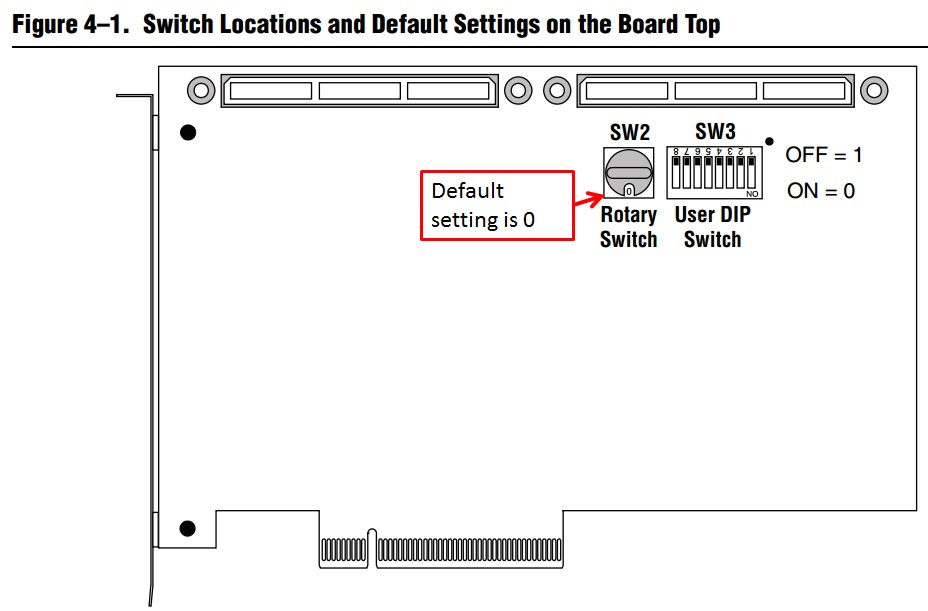
\includegraphics[scale=0.5]{sw1}\\
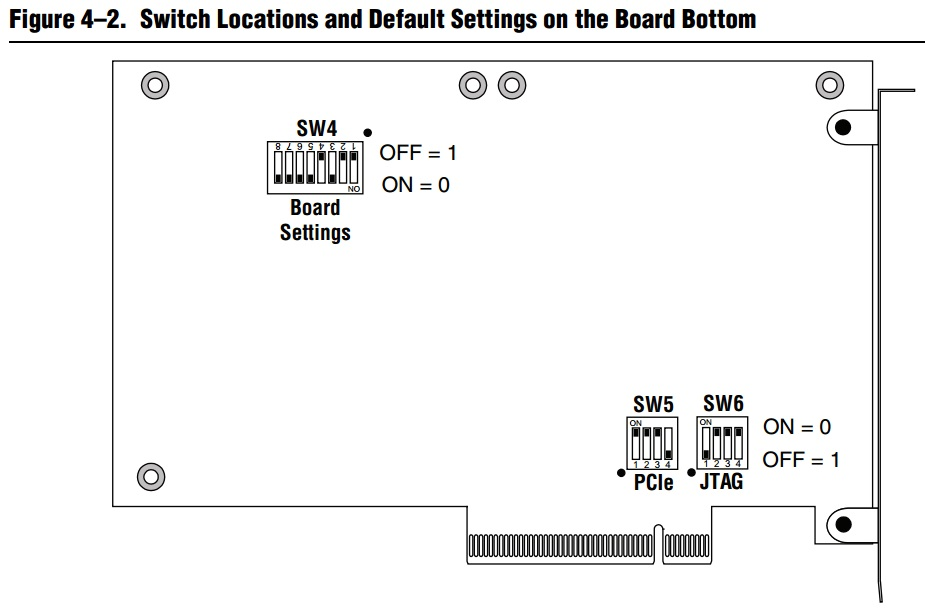
\includegraphics[scale=0.5]{sw2}\\
\subsubsection*{Connect USB Blaster cable and power on board}
Connect USB type B connector to USB port on board and type A connector to OpenCPI development host. Power on board with the external power supply provided with the kit.\par\smallskip
\noindent Enter a terminal and source the OpenCPI environment for x86. Run the following script to test the JTAG connection: opencpi/hdl/scripts/probeJtag\par\smallskip
\noindent The output should look like this:\par\smallskip
\noindent\terminaloutput{==== Probing for Altera JTAG ports:\\Found cable "USB-Blaster [3-2]" with serial number "91d28408"\\==== Probing for Xilinx JTAG ports:\\Discovered ports are:\\Look at /tmp/ocpibitstream5211.1.* for details.}\par\bigskip
\noindent For the purposes of this guide, ignore any messages related to Xilinx.\par\medskip
\noindent If the output doesn't look like this, refer to the USB blaster cable installation for Linux
\subsubsection*{Run loadFlash script}
The loadFlash script is located at opencpi/tools/cdk/scripts. You must pass it a pre-built ALST4 .bitz file generated by OpenCPI and the serial number (in hex) of the JTAG cable from probeJtag script above. This step with take approximately 10 minutes to complete.\par\bigskip
\noindent{\bf alst4 syntax}\par
\noindent\shellcmd{loadFlash alst4 <OpenCPI Bitstream File> <JTAG\_CABLE\_SERIAL\_NUMBER> }\par\smallskip
\noindent{\bf alst4 output}\par
\noindent\shellcmd{[user@opencpi-test1 scripts]\$ ./loadFlash alst4 /home/user/ocpi/opencpi/hdl/platforms/alst4\slash \\testbias\_alst4\_base.bitz 91d28408}
\terminaloutput{Loading the flash memory on the alst4 platform attached to the JTAG pod with ESN 91d28408\\
Loading from file: /home/user/ocpi/opencpi/hdl/platforms/alst4/testbias\_alst4\_base.bitz\\
Found cable "USB-Blaster [2-1.3]" with serial number 91d28408\\
Using cable "USB-Blaster [2-1.3]" with serial number 91d28408.\\
The bitstream file "/home/user/ocpi/opencpi/hdl/platforms/alst4/testbias\_alst4\_base.bitz" is compressed. Expanding it.\\
Bitstream file decompressed into "/tmp/ocpibitstream5351.sof"\\
Converting bitstream file "/tmp/ocpibitstream5351.sof" to flash format in "/tmp/ocpibitstream5351.flash" \\using sof2flash\\
Loading factory bitstream "/home/user/altera/11.1/kits/stratixIVGX\_4sgx230\_fpga/factory\_recovery\slash \\s4gx230\_fpga\_bup.sof" to use for indirectly writing flash memory.\\
JTAG Loading of the factory bitstream succeeded. Now using it to write the flash.\\
real	1m25.590s\\
user	0m0.801s\\
sys	0m0.591s\\
Flash programming is complete. You must power-cycle the system to use it.}\par\bigskip
\noindent Use the "ocpihdl search" command after power cycling to confirm success.\par
\subsubsection*{Modify Linux kernel boot arguments to reserve PCIE memory}
If you want the Linux OpenCPI driver to use more than 128 KB of RAM, then you will need to reserve a block of memory during the Linux kernel boot, using the memmap paramater. Reference the README in the driver directory of the OpenCPI install location for its usage. Regardless of desired RAM size, all CentOS 7 users are recommended to make the grub2 modifications (for 128 MB) specified therein. Make any grub/grub2 modifications and reboot the development system before continuing.

\subsubsection*{Power down board and set rotary switch to load OpenCPI bitstream from flash}
With the board powered down, set SW2 to 1. See figure above for location of SW2 on board. This setting will cause the board to load the bitstream from the flash location we just programmed.\par
\subsubsection*{Install board into PCIe chassis and verify OpenCPI bitstream loads on power up}
With the development system powered down, install the PCIe card. Reconnect the USB cable and then power on the system. To check the board was installed correctly, enter a terminal and source the OpenCPI environment for x86. Then load the PCIe driver using (requires sudo privileges).\par\bigskip
\noindent\shellcmd{ocpidriver load}\par\bigskip
\noindent Perform a container check using ocpirun -C. The result should look like this:\par\bigskip
\noindent\terminaloutput{[user@opencpi-test1 opencpi]\$ ocpirun -C\\
Available containers:\\
 \#  Model\hspace{6ex} Platform\hspace{3ex}    OS\hspace{5ex}     OS Version\hspace{1ex}  Name\\
 0  rcc\hspace{9ex}   x86\_64\hspace{5ex}      linux\hspace{2ex}  c6\hspace{10ex}          rcc0\\
 1  hdl\hspace{9ex}   alst4\hspace{29ex}                          PCI:0000:02:00.0
}
\section*{Known Issue}
See alst4\_getting\_started\_guide.pdf ``Known Issues'' section for known alst4 issues.
\section*{ALST4 Card Support}
The OpenCPI alst4 platform includes support for use of the Zipper/Myriad RF card in one or both HSMC slots on the Stratix IV board. Note that for proper function, the hardware modifications specified in \cite{zipper_mods} are necessary. If using a Zipper/Myriad RF with the alst4, ensure that the Myriad RF card is connected to the Zipper via HSMC.

\pagebreak
  \begin{thebibliography}{1}

  \bibitem{zipper_mods} Required Modifications for Myriad-RF 1 and Zipper Daughtercards\\
	 Required\_Modifications\_for\_Myriad-RF\_1\_Zipper\_Daughtercards.pdf (included in cards doc directory)

  \end{thebibliography}

\end{document}
